\documentclass[letterpaper,10pt,conference]{ieeeconf}
%\documentclass[a4paper,10pt,conference]{ieeeconf}

% This command is only needed if you want to use the \thanks command
\IEEEoverridecommandlockouts 

% See the \addtolength command later in the file to balance the column lengths
% on the last page of the document
\overrideIEEEmargins

\usepackage{graphicx} % for pdf, bitmapped graphics files
%\usepackage{epsfig} % for postscript graphics files
%\usepackage{mathptmx} % assumes new font selection scheme installed
%\usepackage{times} % assumes new font selection scheme installed
%\usepackage{amsmath} % assumes amsmath package installed
%\usepackage{amssymb}  % assumes amsmath package installed
\usepackage{placeins} % for \FloatBarrier

% define some more useful macros
\newcommand{\fref}[1]{Fig.~\ref{#1}}
\newcommand{\eref}[1]{(\ref{#1})}
\newcommand{\tref}[1]{Table~\ref{#1}}
\newcommand{\sref}[1]{Section~\ref{#1}}

% do headery stuff
\title{\LARGE\bf Simulating Nailfold Capillaroscopy Sequences\\to Evaluate Algorithms for Blood Flow Estimation}
%\author{P. A. Tresadern, M. Berks, C. J. Taylor, A. K. Murray, G. Dinsdale and A. L. Herrick%
\author{P. A. Tresadern, M. Berks, A. K. Murray, G. Dinsdale, C. J. Taylor and A. L. Herrick%
\thanks{This work was generously supported by The Wellcome Trust.}%
\thanks{P. A. Tresadern, M. Berks and C. J. Taylor are with the Centre for Imaging Sciences, University of Manchester, United Kingdom M13 9PT. A. K. Murray, G. Dinsdale and A. L. Herrick are with the Institute of Inflammation and Repair, University of Manchester, United Kingdom M13 9PT. Corresponding author: philip.tresadern@manchester.ac.uk}%
}

% define some useful macros
\usepackage{xspace}
\makeatletter
\DeclareRobustCommand\onedot{\futurelet\@let@token\@onedot}
\def\@onedot{\ifx\@let@token.\else.\null\fi\xspace}
\def\eg{\emph{e.g}\onedot} \def\Eg{\emph{E.g}\onedot}
\def\ie{\emph{i.e}\onedot} \def\Ie{\emph{I.e}\onedot}
\def\cf{\emph{c.f}\onedot} \def\Cf{\emph{C.f}\onedot}
\def\etc{\emph{etc}\onedot} \def\vs{\emph{vs}\onedot} 
\def\wrt{w.r.t\onedot} \def\dof{d.o.f\onedot}
\def\pdf{p.d.f\onedot}
\def\etal{\emph{et al}\onedot}
\makeatother

\def\figpath{./fig}

\newlength{\figwidth}
\newlength{\figheight}


\begin{document}

\maketitle
\thispagestyle{empty}
\pagestyle{empty}


\begin{abstract}
The effects of systemic sclerosis (SSc) -- a disease of the connective tissue causing blood flow problems that can require amputation of the fingers -- can be observed indirectly by imaging the capillaries at the nailfold, though taking quantitative measures such as blood flow to diagnose the disease and monitor its progression is not easy. Optical flow algorithms may be applied, though without ground truth (\ie~known blood flow) it is hard to evaluate their accuracy.

We propose an image model that generates realistic capillaroscopy videos with known flow, and use this model to quantify the effect of flow rate, cell density and contrast (among others) on estimated flow. This resource will help researchers to design systems that are robust under real-world conditions.
\end{abstract}


\section{Introduction}
Systemic sclerosis (SSc) is a disease of the connective tissue that causes fibrosis and vascular problems leading to digital ulcers or, in extreme cases, gangrene requiring amputation of the fingers. Prevalence in the US adult population is around 250 per million, with an incidence rate of approximately 20 new cases per million per year~\cite{Mayes_etal_AR03}. Due to limited long-term clinical data, however, there are few effective treatments.

There is, therefore, a need for systems that can diagnose disease early and measure its progression over time, for example in response to drug treatment. Of the techniques for assessing systemic sclerosis~\cite{Murray_etal_AR09}, the gold standard is \emph{nailfold capillaroscopy}: taking images, through a microscope, of the capillaries that lie flush with the skin close to the base of the fingernail (\fref{fig_example_images}a). From these images, we can measure capillary shape, size and density; detect abnormalities and haemorrhages; and observe blood flow in video sequences.

Capillaroscopy is attractive because it is non-invasive and relatively cheap. Capturing high quality images for quantitative assessment with current systems, however, requires training and expertise, and can be time-consuming. This limits research that depends on measuring capillary properties.


\subsection{Related Work}
Properties such as vessel density and morphology can be measured manually from capillaroscopy images~\cite{Anderson_etal_JRh05} using software that combines individual images to create a panorama of the whole nailbed and enhances the visual appearance of the vessels~\cite{Allen_etal_MICCAI99,Allen_etal_BMVC98}. Recent software has automated the measurement process for images of a given quality~\cite{Feng_PhD09,Paradowski_etal_KES09}.

One measurement of interest is blood flow velocity, which can vary rapidly over time. Though efforts have been made to estimate the accuracy of image-based measurements with respect to other computerized solutions~\cite{Mawson_Shore_JMET98} or between different image-based methods~\cite{Wu_etal_MR09}, such evaluations are limited by a lack of ground truth flow values. Although using simulated images to evaluate flow estimation has recently been proposed, sequences generated currently lack realism~\cite{Huang_etal_MR10}.

Image-based flow methods are typically based on one of two paradigms: optical flow~\cite{Horn_Schunk_AI81} exploits differential properties of images of a dynamic scene captured close together in time, whereas region matching methods~\cite{Lucas_Kanade_IUW81} use local search over a neighbourhood and are good for dealing with large motions. The two approaches are complementary, though effort has been made to combine their strengths~\cite{Bruhn_etal_IJCV05}. All can be evaluated using synthetic sequences~\cite{Barron_etal_IJCV94} or real data, captured under highly controlled conditions with near-perfect ground truth~\cite{Baker_etal_IJCV11}.

\begin{figure}
\centering
\resizebox{\columnwidth}{!}{
\setlength{\figheight}{0.25\textheight}
\begin{tabular}{@{}c c c@{}}
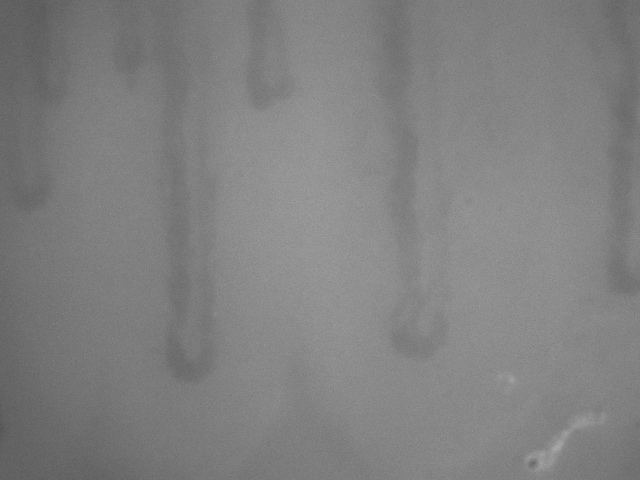
\includegraphics[height=\figheight]{\figpath/real_frame} &
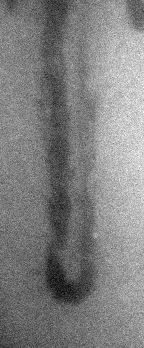
\includegraphics[height=\figheight]{\figpath/real_cap_eq} &
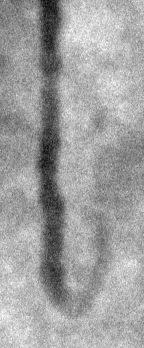
\includegraphics[height=\figheight]{\figpath/fake_cap_eq} \\
(a) & (b) & (c)
\end{tabular}}
%
\caption{Capillaroscopy images: %
(a) Frame from a real capillaroscopy sequence%
%, overlaid with vertical component of estimated blood flow%
; (b) capillary loop from the sequence%
; (c) synthetic capillary generated by our system.
The capillary loops in (b) and (c) have been rescaled to enhance contrast.}
\label{fig_example_images}
\end{figure}



\subsection{Our Objectives}
Our aim is to develop a system that will offer three main benefits to the clinic: images will be quick and easy to capture, using modern cameras with automated motion control; blood vessels in the image will be detected, segmented and measured automatically to give objective and quantitative measures of abnormality; and blood flow will be measured using image processing to provide complementary, dynamic data. These features will allow our capillaroscopy system to be rolled out more widely within healthcare systems.

\begin{figure*}[t]
\centering
\setlength{\figwidth}{0.10\textwidth}
\begin{tabular}{c c c c c c}
  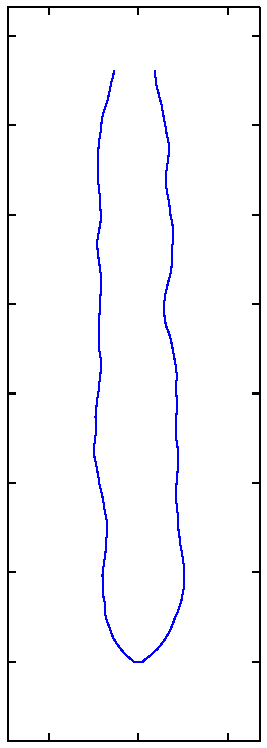
\includegraphics[width=\figwidth]{\figpath/path_points} &
  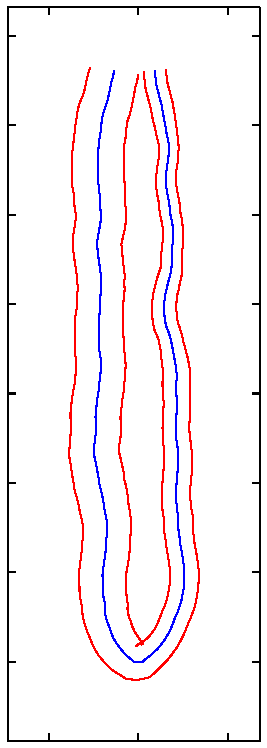
\includegraphics[width=\figwidth]{\figpath/edge_points} &
  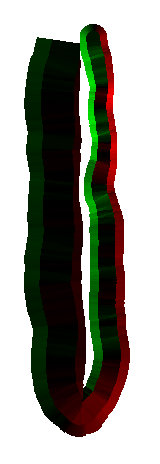
\includegraphics[width=\figwidth]{\figpath/u_gt}
  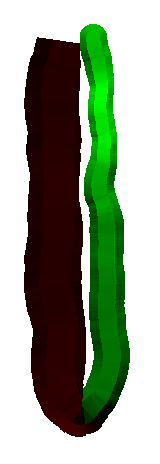
\includegraphics[width=\figwidth]{\figpath/v_gt} &
  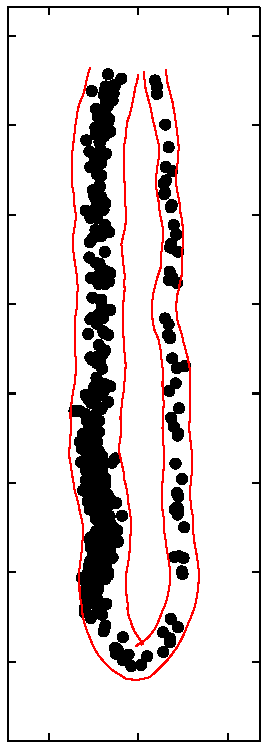
\includegraphics[width=\figwidth]{\figpath/cells_positions} &
  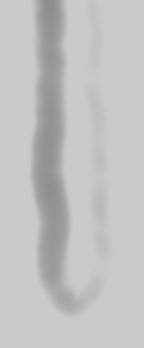
\includegraphics[width=\figwidth]{\figpath/clean} &
  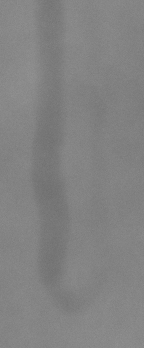
\includegraphics[width=\figwidth]{\figpath/fake_cap} \\
  (a) & (b) & (c) & (d) & (e) & (f)
\end{tabular}
%
\caption{Image synthesis process: (a) path of the vessel centre; (b) edges of the venous and arterial limb; (c) horizontal and vertical flow fields, respectively; (d) blood cell positions along the vessel centre; (e) synthetic image, before adding noise artefacts; (f) final synthetic image. For the flow fields in (c), hue indicates the direction of flow over the sequence (green is right/down, red is left/up) and intensity is proportional to flow rate (black indicates zero flow).}
\label{fig_image_generation}
\end{figure*}


Here we assess the efficacy of algorithms for measuring blood flow in capillaroscopy sequences by developing a model that generates synthetic sequences of capillary blood flow, complete with exact flow values at every pixel.%
\footnote{Example sequences are available at the time of writing from %
http://personalpages.manchester.ac.uk/staff/philip.tresadern/proj\_nailfold.htm}%
These values can then be compared with those estimated from the image data to quantify error in estimated flow with respect to parameters such as flow velocity, cell density and noise.


\section{Methods}

\subsection{Generating Images}
In generating an image sequence, we first define the capillary shape and its boundaries. Healthy capillaries have a characteristic `hairpin' shape: the capillary is largely straight with a `u-turn' at its apex. We therefore generate each side of the vessel path by tracing the locus of a point that travels with a constant vertical velocity and a horizontal velocity that falls to zero, plus a small random components so that the vessel is not perfectly straight (\fref{fig_image_generation}a).

A capillary has two limbs: a thin, arterial limb carrying blood from the heart; and a thicker, venous limb that carries blood back to the heart. We generate the edges of the two limbs using a stochastic process whereby we define the width at the apex and allow it either to grow or shrink to a constant value, with a small random component to model natural variation in width along the length of the vessel (\fref{fig_image_generation}b).

Next, we map the vessel centre and edges to a pixel grid where we can define a flow direction and magnitude at every pixel. Pixels that lie between the vessel walls are assigned a flow vector whose direction is parallel to the vessel path at its closest point, and whose magnitude is inversely proportional to the cross sectional area of the vessel at that point (such that flow is conserved along the length of the vessel). Pixels that lie just outside of the vessel wall are assigned a similar flow vector, plus a component toward the centre of the vessel to simulate collisions with the vessel wall. All other pixels are assigned a zero flow vector (\fref{fig_image_generation}c).

Now that we have the vessel structure and flow at every point, we can simulate the motion of individual blood cells over time. To do so, we choose a fixed number of blood cells and initialize their positions at sampled points along the centre of the vessel. At each time instant for every blood cell, we interpolate the flow vector from the pixel grid at the cell's position and apply the corresponding motion (plus a small random motion component) to the blood cell to compute its position at the following time step (\fref{fig_image_generation}d). By iterating this process, we generate a sequence of blood cell positions for any number of frames.

In a capillaroscopy image, an individual blood cell appears as a dark, blurry blob that we approximate with a Gaussian in the image. To simulate the appearance of plasma (gaps in the blood flow), we darken the image by a random amount for every cell. Next, we mask out pixels that lie outside the vessel boundary, and smooth the image. We then apply an offset and scaling to this `clean' image to approximate the brightness and contrast of a typical capillaroscopy image (\fref{fig_image_generation}e).

Finally, we add artefacts to the image to simulate common causes of image degradation in capillaroscopy. First, we add a random but spatially correlated background texture to the image to simulate slight intensity variation in the underlying tissue.%
\footnote{This texture was generated using Matlab code provided by Peter Kovesi.%
\\http://www.csse.uwa.edu.au/~pk/Research/MatlabFns/Misc/noiseonf.m}
We then modulate the brightness and contrast of the image randomly over the sequence to approximate illumination changes. Last, we add a small random translation to every image to simulate `shake' that is almost unavoidable when viewing live structures at a microscopic scale. The final result is an image sequence that is qualitatively similar to a real capillaroscopy sequence (\fref{fig_image_generation}f).


\subsection{Estimating Flow}
Given a sequence of images, real or synthetic, we can apply optical flow methods to estimate blood flow for every pixel at every point in time. We assume, for now, that the images in the sequence have been registered to remove any small translations between frames; synthetic sequences can be generated such that this is so, whereas real sequences must go through a registration process~\cite{Zitova_Flusser_IVC03}. We also assume that brightness (mean intensity) and contrast (intensity variance) are largely constant over the sequence, which also can be achieved by design or image post-processing.

In its simplest form, optical flow assumes that a pixel associated with a moving object will maintain its brightness over time such that, by a first order Taylor expansion,
%
\begin{eqnarray}
I(x, y, t) 
&=& I(x+dx, y+dy, t+dt) \\
&\approx& I(x, y, t) + \frac{\partial I}{\partial x} \frac{dx}{dt} 
							 + \frac{\partial I}{\partial y} \frac{dy}{dt} 
							 + \frac{\partial I}{\partial t} \\
\Rightarrow
0 &\approx& I_x u + I_y v + I_t,
\end{eqnarray}
%
\noindent where $I_x$ is the partial derivative $\partial I / \partial x$ (and likewise for $y$ and $t$) that can be estimated by finite differencing; the flow vector components $u = dx/dt$ and $v = dy/dt$ are the quantities we want to know.

This one equation with two unknowns has an infinite number of solutions, since any motion parallel to an edge is unobservable (known as the `aperture effect'). Though global contraints can be applied to ensure a smoothly varying flow field~\cite{Horn_Schunk_AI81}, we instead pool measurements over a small window (\eg~$3 {\times} 3$ pixels) to increase the number of constraints on $u$ and $v$. Because this is essentially a linear regression, we can also use an eigenanalysis to identify patches where the solution is poorly constrained and even quantify the uncertainty in the estimated flow directions.

Estimating flow from a single pair of noisy images, however, is error-prone. We therefore average over every consecutive pair of frames in the sequence to obtain the mean flow at every pixel. Alternatively, we could compute an approximate distribution of flow over time for every pixel and examine the properties of the distribution, such as variance which reflects uncertainty.


\subsection{Experiments}
The purpose of creating synthetic capillaroscopy sequences is to assess the accuracy of the estimated blood flow under different conditions. In particular, we want to know when the optical flow algorithm will work well or break down, and to quantify the effect of different parameters. We therefore generated sequences for various values of flow rate, cell density, brightness variation, contrast variation, translational `shake' and additive Gaussian noise. For the purposes of this quantitive study, we did not add a background texture.

To quantify error, we computed flow at every pixel in every consecutive pair of images over the sequence. We then computed statistics for every pixel, such as the mean flow vector and its variance (independently in $u$ and $v$) over the sequence. Finally, we computed the mean absolute error (MAE) in $u$ and $v$ between the estimated flow and the ground truth over the whole image. All sequences contained $180$ frames, equivalent to three seconds of video at $60$ frames per second (the frame rate of our hardware). Unless stated otherwise, baseline background brightness is $120$ grey levels and contrast (\ie~the difference between the lightest and darkest pixels) is $16$ grey levels.

\section{Results}
\begin{figure}
\centering
\resizebox{\columnwidth}{!}{
\begin{tabular}{c c}
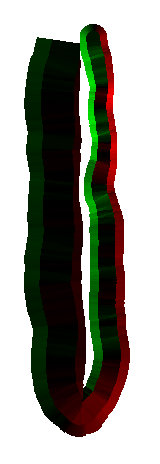
\includegraphics[width=0.25\columnwidth]{\figpath/u_gt}
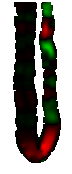
\includegraphics[width=0.25\columnwidth]{\figpath/u_est} &
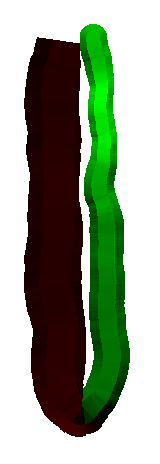
\includegraphics[width=0.25\columnwidth]{\figpath/v_gt}
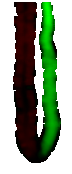
\includegraphics[width=0.25\columnwidth]{\figpath/v_est} \\
(a) & (b)
\end{tabular}}
%
\caption{Qualitative comparison of true flow field with that estimated from optical flow in the (a) horizontal and (b) vertical directions. Hue indicates the direction of flow over the sequence (green is right/down, red is left/up) and intensity is proportional to flow rate (black indicates zero flow).}
\label{fig_flow_results_synth}
\end{figure}

\begin{figure}
\centering
\resizebox{\columnwidth}{!}{
\begin{tabular}{@{} c c @{}}
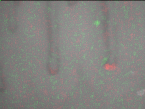
\includegraphics[width=0.5\columnwidth]{\figpath/real_flow/u_overlay} &
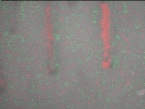
\includegraphics[width=0.5\columnwidth]{\figpath/real_flow/v_overlay} \\
(a) & (b)
\end{tabular}}
%
\caption{Real image (\fref{fig_example_images}) overlaid with estimated image flow in the (a) horizontal and (b) vertical directions. Because flow magnitude is not available for this real sequence, the colouring instead indicates the direction of flow over the sequence: green is right/down; red is left/up. The intensity denotes the proportion of the sequence in the given direction. The regions of flow in the two vessels are clear.}
\label{fig_flow_results}
\end{figure}


Qualitatively, the flow in a slow-moving column of blood was recovered well, particularly in the vertical direction in which most of the flow took place (\fref{fig_flow_results_synth}). We also applied the algorithm to registered sets of real images, though we have no ground truth and can present only the estimated \emph{direction} of flow; it would seem, however, that the algorithm detected the regions of flow in the sequence (\fref{fig_flow_results}).

\begin{figure}
\centering
\setlength{\figwidth}{0.5\columnwidth}
\resizebox{\columnwidth}{!}{
\begin{tabular}{c c}
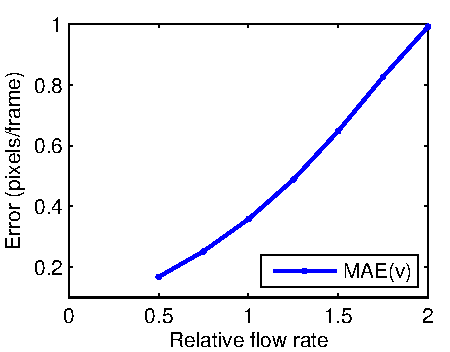
\includegraphics[width=\figwidth]{\figpath/flowrate} &
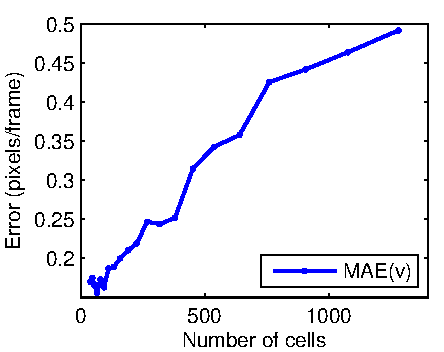
\includegraphics[width=\figwidth]{\figpath/n_cells} \\
(a) & (b) \\
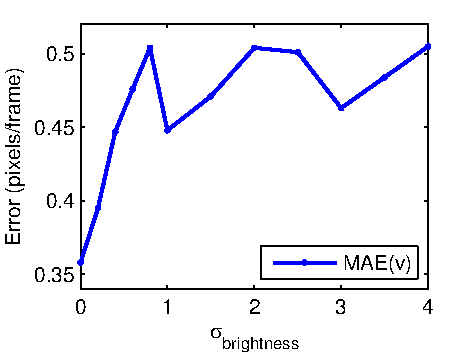
\includegraphics[width=\figwidth]{\figpath/brightness_sigma} &
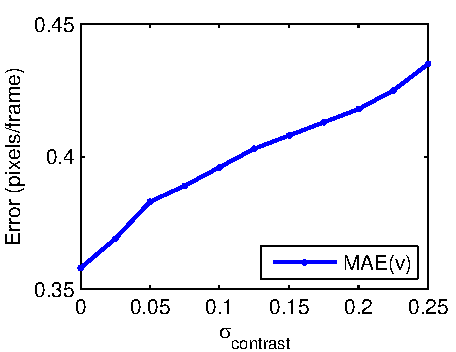
\includegraphics[width=\figwidth]{\figpath/contrast_sigma} \\
(c) & (d)
\end{tabular}}
%
\caption{Mean Absolute Error (MAE) in the vertical direction with respect to (a) relative flow rate, (b) number of simulated cells, (c) brightness variation and (d) contrast variation.}
\label{fig_flow_graphs_synth}
\end{figure}


When comparing quantitative error rates with respect to vertical flow magnitude (since this is where most flow takes place), mean absolute error varied approximately linearly with respect to flow rate (\fref{fig_flow_graphs_synth}a). With respect to the number of cells (or cell density), error increased with the number of cells simulated (\fref{fig_flow_graphs_synth}b).

Small random variations in brightness (\fref{fig_flow_graphs_synth}c), `shake' and added Gaussian noise (not shown) increased the error rapidly initially before reaching a plateau of approximately $0.5$ to $0.6$ pixels per frame, where further increases in the size of the variations had a much smaller effect.

Contrast variation, being a multiplicative (rather than additive) parameter has wider influence such that error contiues to increase linearly within the range tested (\fref{fig_flow_graphs_synth}d).


\section{Discussion}
Our results suggest that flow rate is the most critical parameter that affects error. This is not surprising because optical flow estimation algorithms consider only a small neighbourhood around any pixel at a given time, such that algorithms will be ineffective for flows greater than some value. This can be addressed in two ways: increase the frame rate of capture hardware; or apply a hierarchical pyramid scheme whereby the flow that is estimated for each spatially subsampled image is used to initialize flow estimation at the next level of the pyramid.

Flow is most accurately measured in regions of high image gradient (\ie~edges) so the \emph{cell density} in the image also has an effect: as density increases, cells overlap and obscure each other's boundaries. Cell density, however, is largely out of our control which could affect the feasibility of estimating blood flow by capillaroscopy alone. Other imaging methods (\eg~OCT) may achieve accurate estimates, though this makes the system more complex and expensive, and requires a difficult data fusion step.

Random variation in brightness introduces errors in flow estimates via the temporal derivatives, whereas variation in contrast, translational noise (`shake') and Gaussian noise affect both spatial and temporal derivatives. Brightness and contrast changes can, however, be normalized to a large degree by applying a global transformation to every image that matches the brightness and contrast to a reference image (\eg~the first) for every frame. Shake, or `jitter', in the sequence can be reduced by applying image registration~\cite{Zitova_Flusser_IVC03} to the sequence before computing optical flow. 


%\newpage
\section{Conclusion}
We have presented a model that simulates capillaroscopy sequences, from which we evaluate algorithms for estimating blood flow under various conditions. The results suggest that apparent flow rate (\ie~distance travelled per frame) has the greatest effect, whereas the increase in error is limited for other parameters such as brightness variation.

Though the model has promise in designing and developing algorithms for estimating flow, it may have uses beyond this task. Because the model includes a parameter to add random translations (that may also be correlated over time by smoothing), we can simulate the effect of errors in registration to evaluate the accuracy of registration algorithms. Our model of image synthesis is also well-suited to generating annotated training data from which optical flow parameters can be learnt rather than prescribed~\cite{Sun_etal_ECCV08}.


\section*{Acknowledgments}
This work was supported by The Wellcome Trust.

%\def\bibpath{s:/bib}
%\bibliographystyle{ieeetran}
%\bibliography{%
%_aliases,%
%local,papers_by_year,nailfold}

\begin{thebibliography}{10}
\providecommand{\url}[1]{#1}
\csname url@rmstyle\endcsname
\providecommand{\newblock}{\relax}
\providecommand{\bibinfo}[2]{#2}
\providecommand\BIBentrySTDinterwordspacing{\spaceskip=0pt\relax}
\providecommand\BIBentryALTinterwordstretchfactor{4}
\providecommand\BIBentryALTinterwordspacing{\spaceskip=\fontdimen2\font plus
\BIBentryALTinterwordstretchfactor\fontdimen3\font minus
  \fontdimen4\font\relax}
\providecommand\BIBforeignlanguage[2]{{%
\expandafter\ifx\csname l@#1\endcsname\relax
\typeout{** WARNING: IEEEtran.bst: No hyphenation pattern has been}%
\typeout{** loaded for the language `#1'. Using the pattern for}%
\typeout{** the default language instead.}%
\else
\language=\csname l@#1\endcsname
\fi
#2}}

\bibitem{Mayes_etal_AR03}
M.~Mayes, J.~Lacey, J.~Beebe-{D}immer, B.~Gillespie, B.~Cooper, T.~Laing, and
  D.~Schottenfeld, ``Prevalence, incidence, survival, and disease
  characteristics of systemic sclerosis in a large us population,''
  \emph{Arthritis Rheum}, vol.~48, pp. 2246--55, 2003.

\bibitem{Murray_etal_AR09}
A.~K. Murray, T.~L. Moore, J.~B. Manning, C.~Taylor, C.~E.~M. Griffiths, and
  A.~L. Herrick, ``Noninvasive imaging techniques in the assessment of
  scleroderma spectrum disorders,'' \emph{Arthritis Rheum}, vol.~61, no.~8, pp.
  1103--11, 2009.

\bibitem{Anderson_etal_JRh05}
M.~E. Anderson, P.~D. Allen, T.~Moore, V.~Hillier, C.~J. Taylor, and A.~L.
  Herrick, ``Computerized nailfold video capillaroscopy -- {A} new tool for
  assessment of raynaud�s phenomenon,'' \emph{J Rheumatology}, pp. 841--848,
  2005.

\bibitem{Allen_etal_MICCAI99}
P.~D. Allen, C.~J. Taylor, A.~L. Herrick, and T.~Moore, ``Image analysis of
  nailfold capillary patterns from video sequences,'' in \emph{Proc. Int. Conf.
  on Medical Imaging Computing and Computer Assisted Intervention}, 1999.

\bibitem{Allen_etal_BMVC98}
------, ``Enhancement of temporally variable features in nailfold capillary
  patterns,'' in \emph{Proc. British Machine Vision Conf.}, 1998.

\bibitem{Feng_PhD09}
K.~Feng, ``Automatic nailfold capillary measurement and analysis,'' Ph.D.
  dissertation, 2009.

\bibitem{Paradowski_etal_KES09}
M.~Paradowski, H.~Kwasnicka, and K.~Borysewicz, ``Capillary blood vessel
  tortuosity measurement using graph analysis,'' in \emph{KES}, vol.~2, 2009,
  pp. 135--142.

\bibitem{Mawson_Shore_JMET98}
D.~M. Mawson and A.~C. Shaw, ``Comparison of {C}api{F}low and frame by frame
  analysis for the assessment of capillary red blood cell velocity,'' \emph{J
  Medica Eng Tech}, vol.~22, no.~2, pp. 53--63, 1998.

\bibitem{Wu_etal_MR09}
C.-C. Wu, G.~Zhang, T.-C. Huang, and K.-P. Lin, ``Red blood cell velocity
  measurements of complete capillary in finger nail-fold using optical flow
  estimation,'' \emph{Microvascular Research}, vol.~78, pp. 319--324, 2009.

\bibitem{Huang_etal_MR10}
T.-C. Huang, W.-C. Lin, C.-C. Wu, G.~Zhang, and K.-P. Lin, ``Experimental
  estimation of blood flow velocity through simulation of intravital
  microscopic imaging in micro-vessels by different image processing methods,''
  \emph{Microvascular Research}, vol.~80, pp. 477--483, 2010.

\bibitem{Horn_Schunk_AI81}
B.~K.~P. Horn and B.~G. Schunk, ``Determining optical flow,'' \emph{Artif.
  Intell.}, vol.~17, pp. 185--203, Aug. 1981.

\bibitem{Lucas_Kanade_IUW81}
B.~Lucas and T.~Kanade, ``An iterative image registration technique with an
  application to stereo vision,'' in \emph{Proc. Image Understanding Workshop},
  1981.

\bibitem{Bruhn_etal_IJCV05}
A.~Bruhn, J.~Weickert, and C.~Schnorr, ``Lucas/{K}anade meets {H}orn/{S}chunck:
  {C}ombining local and global optic flow methods,'' \emph{Int. J. Comput.
  Vis.}, vol.~61, no.~3, pp. 211--231, 2005.

\bibitem{Barron_etal_IJCV94}
J.~L. Barron, D.~J. Fleet, and S.~S. Beauchemin, ``Performance of optical flow
  techniques,'' \emph{Int. J. Comput. Vis.}, vol.~12, no.~1, pp. 43--77, 1994.

\bibitem{Baker_etal_IJCV11}
S.~Baker, D.~Scharstein, J.~P. Lewis, S.~Roth, M.~J. Black, and R.~Szeliski,
  ``A database and evaluation methodology for optical flow,'' \emph{Int. J.
  Comput. Vis.}, vol.~92, pp. 1--31, 2011.

\bibitem{Zitova_Flusser_IVC03}
B.~Zitova and J.~Flusser, ``Image registration methods: a survey,'' \emph{Image
  Vision Comput.}, vol.~21, pp. 977--1000, 2003.

\bibitem{Sun_etal_ECCV08}
D.~Sun, S.~Roth, J.~P. Lewis, and M.~J. Black, ``Learning optical flow,'' in
  \emph{Proc. European Conf. on Computer Vision}, vol.~3, 2008, pp. 83--97.

\end{thebibliography}

\end{document}
